%!TEX program = xelatex

\documentclass[12pt,a4paper]{article}
\usepackage{xeCJK}
\usepackage{amsmath}
\setmainfont{Times New Roman}
\usepackage{setspace}
\usepackage{caption}
\usepackage{graphicx, subfig}
\usepackage{float}
\usepackage{listings}
\usepackage{makecell}
\usepackage{booktabs}
\usepackage{setspace}%使用间距宏包
\usepackage{mathtools}
\usepackage{amsfonts}
\usepackage{tabularx}
\usepackage{amsmath}
    \usepackage{geometry}
        \geometry{margin=1.2in}
    \usepackage{hyperref}
    \usepackage[listings]{tcolorbox}
        \newtcblisting{paste}{%
            title=\texttt{Code Pasting Area},listing only}


\begin{document} 
\title{homework5}
	\author{11611118 郭思源}  



\section{Question 1}
		\begin{spacing}{1.5}
        For the data sets in Problems~\ref{T:hw-5-1}--\ref{T:hw-5-4}, construct a divided difference table. Is smoothing with a low-order polynomial appropriate? If so, choose an appropriate polynomial and fit using the least-squares criterion of best fit. Analyze the goodness of fit by examining appropriate indicators and graphing the model, the data points, and the deviations.
        \end{spacing}
        \begin{enumerate}
            \item\label{T:hw-5-1}
                \begin{tabular}[t]{l|rrrrrrrr}
                    $x$ & 0 & 1 & 2  & 3  & 4   & 5   & 6   & 7   \\ \hline
                    $y$ & 2 & 8 & 24 & 56 & 110 & 192 & 308 & 464 \\
                \end{tabular}
                \begin{paste}
    x = [0, 1, 2, 3, 4, 5, 6, 7];
    y = [2, 8, 24, 56, 110, 192, 308, 464];
                \end{paste}
            \item\label{T:hw-5-2}
                \begin{tabular}[t]{l|rrrrrrrr}
                    $x$ & 0  & 1  & 2  & 3  & 4   & 5   & 6   & 7   \\ \hline
                    $y$ & 23 & 48 & 73 & 98 & 123 & 148 & 173 & 198 \\
                \end{tabular}
                \begin{paste}
    x = [0, 1, 2, 3, 4, 5, 6, 7];
    y = [23, 48, 73, 98, 123, 148, 173, 198];
                \end{paste}
            \item\label{T:hw-5-3}
                \begin{tabular}[t]{l|rrrrrrrr}
                    $x$ & 0 & 1  & 2  & 3  & 4  & 5   & 6   & 7   \\ \hline
                    $y$ & 7 & 15 & 33 & 61 & 99 & 147 & 205 & 273 \\
                \end{tabular}
                \begin{paste}
    x = [0, 1, 2, 3, 4, 5, 6, 7];
    y = [7, 15, 33, 61, 99, 147, 205, 273];
                \end{paste}
            \item\label{T:hw-5-4}
                \begin{tabular}[t]{l|rrrrrrrr}
                    $x$ & 0 & 1   & 2  & 3  & 4   & 5    & 6    & 7     \\ \hline
                    $y$ & 1 & 4.5 & 20 & 90 & 403 & 1808 & 8103 & 36316 \\
                \end{tabular}
                \begin{paste}
    x = [0, 1, 2, 3, 4, 5, 6, 7];
    y = [1, 4.5, 20, 90, 403, 1808, 8103, 36316];
                \end{paste}
        \end{enumerate}
        \newpage

        \begin{spacing}{1.5}
        \subsection{Problem 1}
        \begin{center}
        \begin{tabular}[t]{l|cccccccc}
            $x$ & 0 & 1 & 2  & 3  & 4   & 5   & 6   & 7   \\ 
            \hline
            $y$ & 2 & 8 & 24 & 56 & 110 & 192 & 308 & 464 \\
        \end{tabular}
        \end{center} 
        $\\$The divided difference table for data:\\
        \begin{center}
        \begin{tabular}[b]{cc|cccc} 
        $x$ & $y$ & $\Delta y$ & $\Delta^2 y$ & $\Delta^3 y$ &$\Delta^4 y$\\
        \hline 
        \makecell{0\\1\\2\\3\\4\\5\\6\\7} & 
        \makecell{2\\8\\24\\56\\110\\192\\308\\464} &
        \makecell{6\\16\\32\\54\\82\\116\\156} &
     	\makecell{5\\8\\11\\14\\17\\20}&
     	\makecell{1\\1\\1\\1\\1}&
     	\makecell{0\\0\\0\\0}
        \end{tabular}
        \end{center}
        
        $\\$So I chose the 3-order polynomial to fit this data set:

        \begin{figure}[htbp]
		\centering
		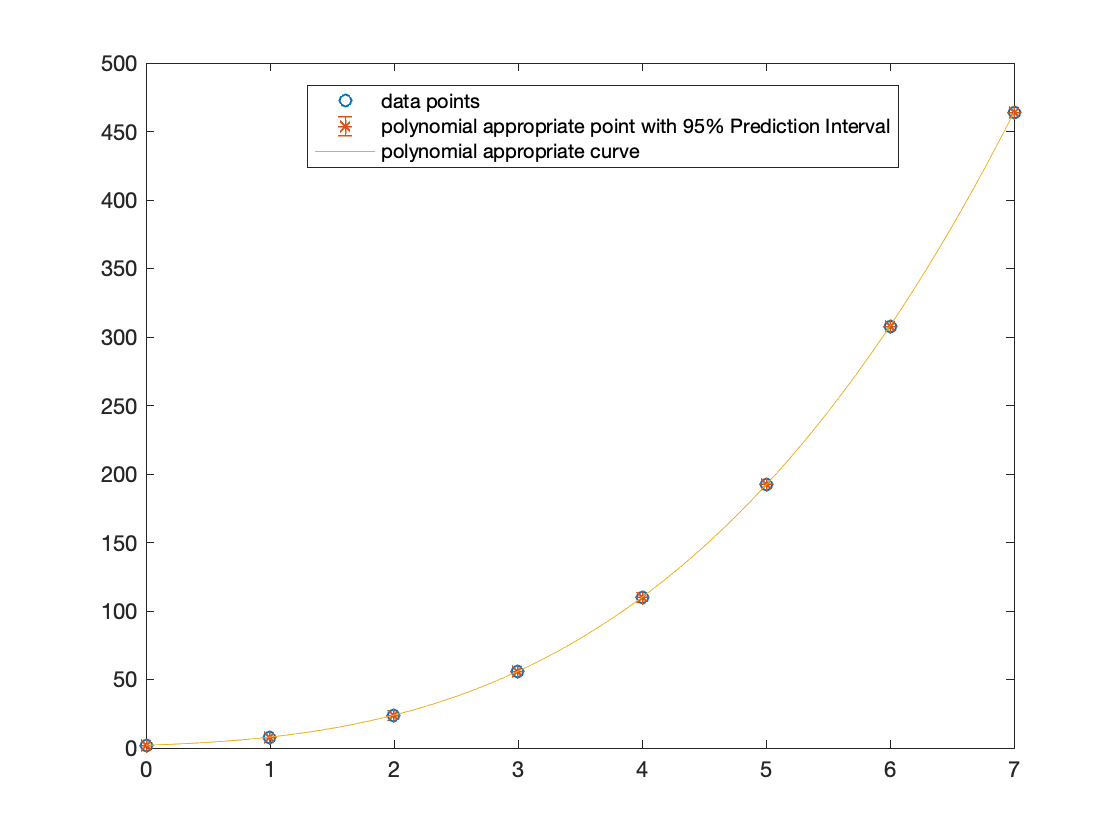
\includegraphics[scale=0.3]{figure/1_1.png}
		\end{figure}


        \newpage
        \subsection{Problem 2}
        \begin{center}
        \begin{tabular}[t]{l|cccccccc}
            $x$ & 0  & 1  & 2  & 3  & 4   & 5   & 6   & 7   \\ 
            \hline
            $y$ & 23 & 48 & 73 & 98 & 123 & 148 & 173 & 198 \\
        \end{tabular}
        \end{center}
        $\\$The divided difference table for data:\\
        \begin{center}
        \begin{tabular}[b]{cc|cc} 
        $x$ & $y$ & $\Delta y$ & $\Delta^2 y$ \\
        \hline 
        \makecell{0\\1\\2\\3\\4\\5\\6\\7} & 
        \makecell{23\\48\\73\\98\\123\\148\\173\\198} &
        \makecell{25\\25\\25\\25\\25\\25\\25} &
     	\makecell{0\\0\\0\\0\\0\\0}
        \end{tabular}
        \end{center}

		$\\$So I chose the 1-order polynomial to fit this data set :

        \begin{figure}[htbp]
		\centering
		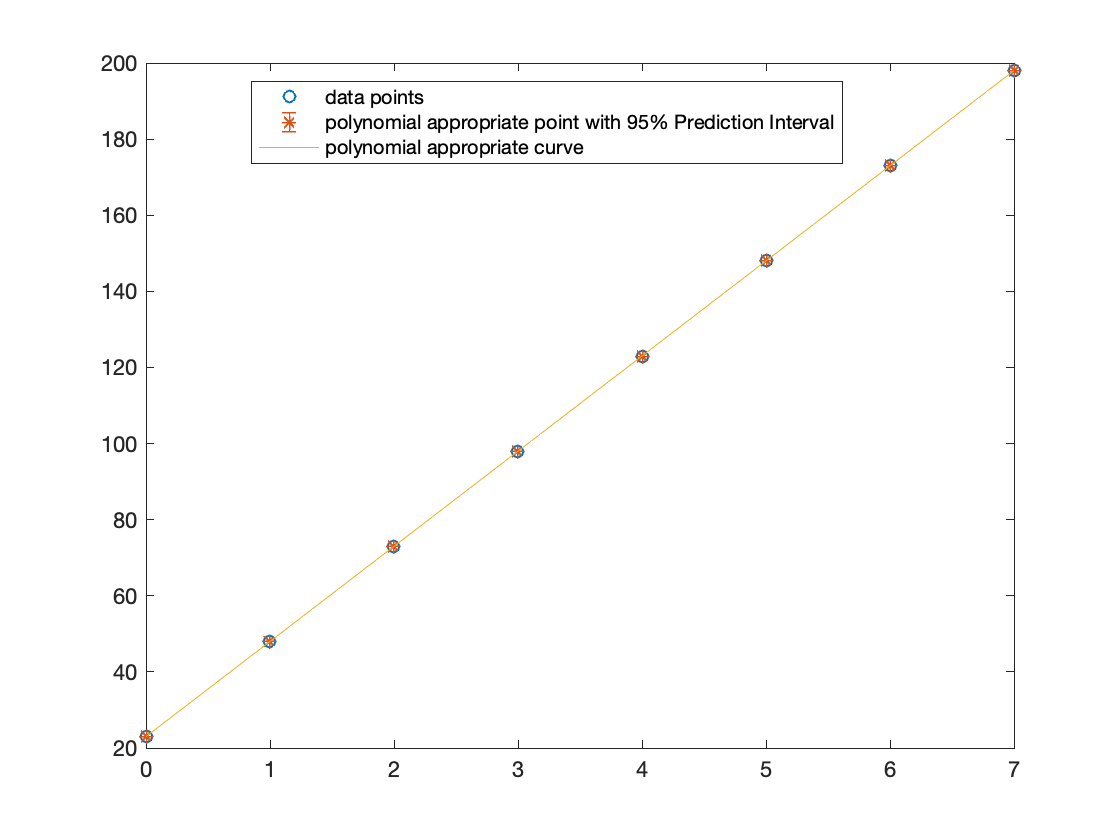
\includegraphics[scale=0.3]{figure/1_2.png}
		\end{figure}




        \newpage
        \subsection{Problem 3}
        \begin{center}
        \begin{tabular}[t]{l|cccccccc}
            $x$ & 0 & 1  & 2  & 3  & 4  & 5   & 6   & 7   \\ 
            \hline
            $y$ & 7 & 15 & 33 & 61 & 99 & 147 & 205 & 273 \\
        \end{tabular}
        \end{center}
        $\\$The divided difference table for data:\\
        \begin{center}
        \begin{tabular}[b]{cc|ccc} 
        $x$ & $y$ & 
        $\Delta y$ & $\Delta^2 y$ & $\Delta^3 y$ \\
        \hline 
        \makecell{0\\1\\2\\3\\4\\5\\6\\7} & 
        \makecell{7\\15\\33\\61\\99\\147\\205\\273} &
        \makecell{8\\18\\28\\38\\48\\58\\68} &
     	\makecell{5\\5\\5\\5\\5\\5}&
     	\makecell{0\\0\\0\\0\\0}
        \end{tabular}
        \end{center}

        $\\$So I chose the 2-order polynomial to fit this data set :

        \begin{figure}[htbp]
		\centering
		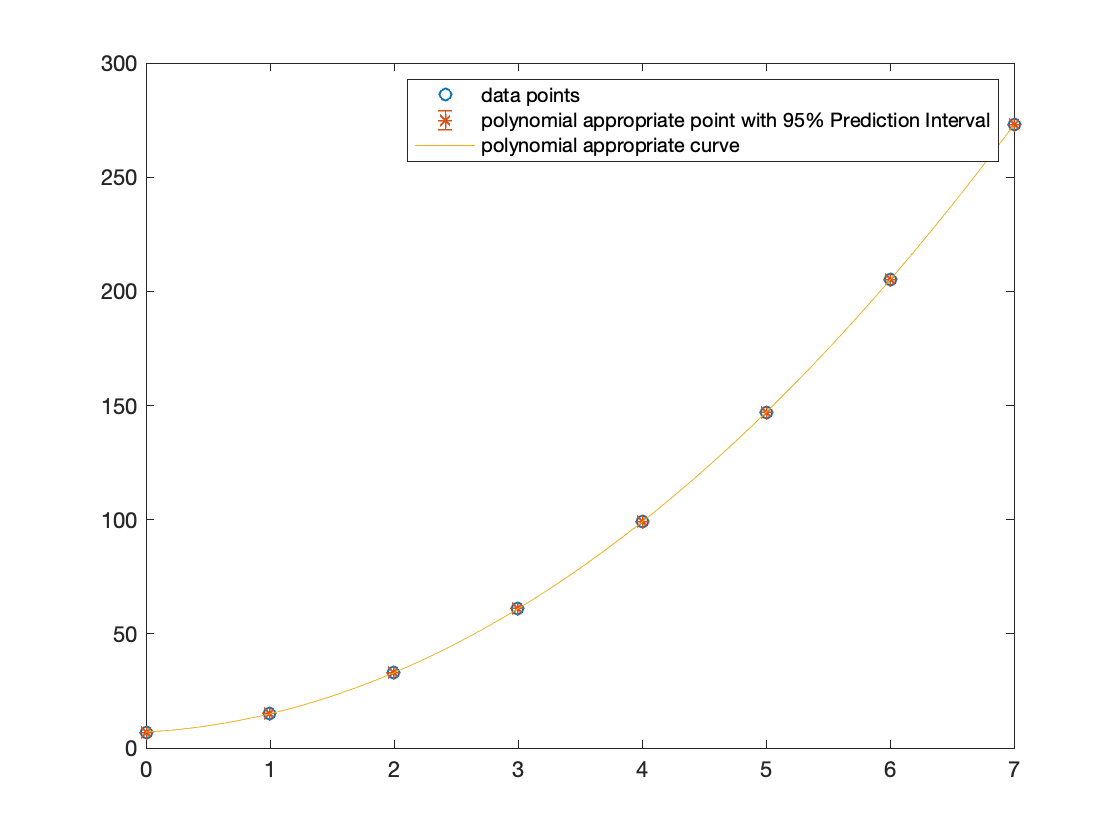
\includegraphics[scale=0.3]{figure/1_3.png}
		\end{figure}


        \newpage
        \subsection{Problem 4}
        \begin{center}
        \begin{tabular}[t]{l|cccccccc}
            $x$ & 0 & 1   & 2  & 3  & 4   & 5    & 6    & 7     \\ 
            \hline
            $y$ & 1 & 4.5 & 20 & 90 & 403 & 1808 & 8103 & 36316 \\
        \end{tabular}
        \end{center}
        $\\$The divided difference table for data:\\
        \begin{center}
        \begin{tabular}[b]{cc|ccccccc} 
        $x$ & $y$ & 
        $\Delta y$ & $\Delta^2 y$ & $\Delta^3 y$ & 
        $\Delta^4 y$ & $\Delta^5 y$ & $\Delta^6 y$ & $\Delta^7 y$\\
        \hline 
        \makecell{0\\1\\2\\3\\4\\5\\6\\7} & 
        \makecell{1\\4.5\\20\\90\\403\\1808\\8103\\36316} &
        \makecell{3.5\\15.5\\70\\313\\1405\\6295\\28213} &
     	\makecell{6\\27.25\\121.5\\546\\2445\\10959}&
     	\makecell{7.0833\\31.417\\141.5\\633\\2838}&
     	\makecell{6.0833\\27.521\\122.87\\551.25}&
     	\makecell{4.2875\\19.071\\85.675}&
     	\makecell{2.4639\\11.101}&
     	\makecell{1.2338}
        \end{tabular}
        \end{center}

        $\\$So I chose the 7-order polynomial to fit this data set :

        \begin{figure}[htbp]
		\centering
		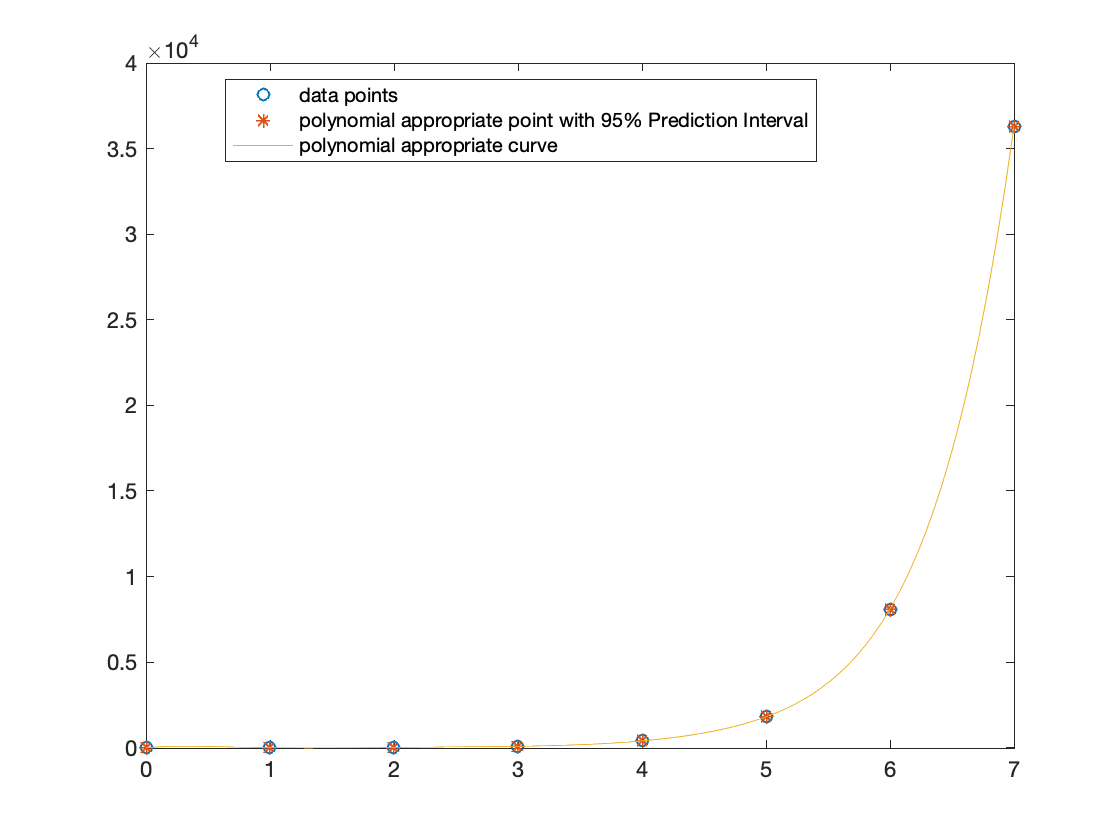
\includegraphics[scale=0.3]{figure/1_4.png}
		\end{figure}
		\end{spacing}



\newpage
\section{Question 2}
		\begin{spacing}{1.5}
        In the following data, $X$ represents the diameter of a ponderosa pine measured at breast height, and $Y$ is a measure of volume---number of board feet divided by 10. Construct a scatterplot of the given data. Is there a trend in the data? Are any of the data points outliers? Construct a divided difference table. Is smoothing with a low-order polynomial appropriate? If so, choose an appropriate polynomial and fit using the least-squares criterion of best fit. Analyze the goodness of fitt by examining appropriate indicators and graphing the model, the data points, and the deviations.
        \end{spacing}

        \begin{center}
            \begin{tabular}{l|cccccccccccccc}
                $X$ & 17 & 19 & 20 & 22 & 23 & 25 & 31  & 32  & 33  & 36  & 37  & 38  & 39  & 41  \\ 
                \hline
                $Y$ & 19 & 25 & 32 & 51 & 57 & 71 & 141 & 123 & 187 & 192 & 205 & 252 & 248 & 294 \\
            \end{tabular}
        \end{center}
        $\\$Remove the outliers form the data set: \\
		\begin{center}
            \begin{tabular}{l|cccccccccccc}
                $X$ & 17 & 19 & 20 & 22 & 23 & 25 & 31  &  36  & 37  & 39  & 41  \\ 
                \hline
                $Y$ & 19 & 25 & 32 & 51 & 57 & 71 & 141 &  192 & 205 & 248 & 294 \\
            \end{tabular}
        \end{center}

        \begin{figure}[htbp]
		\begin{minipage}[t]{0.5\linewidth}
		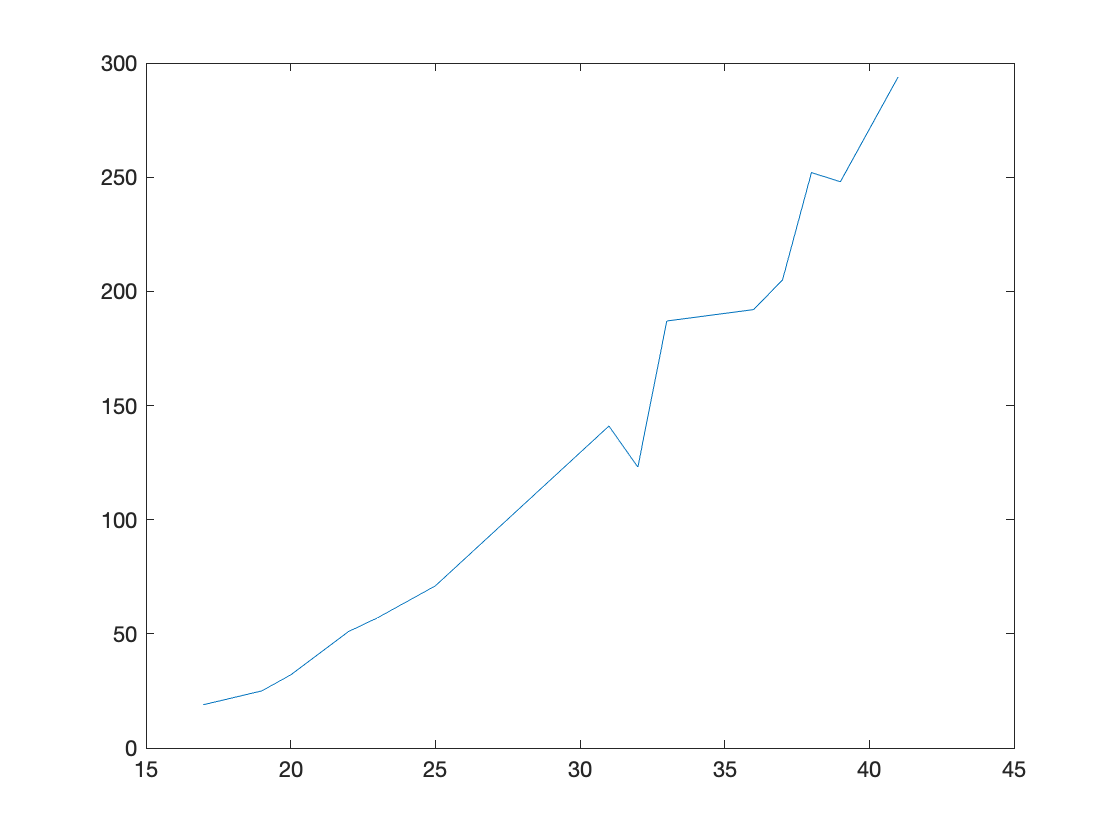
\includegraphics[width=8cm]{figure/2_1.png}
		\caption{Before}
		%\label{fig:side:a}
		\end{minipage}%
		\begin{minipage}[t]{0.5\linewidth}
		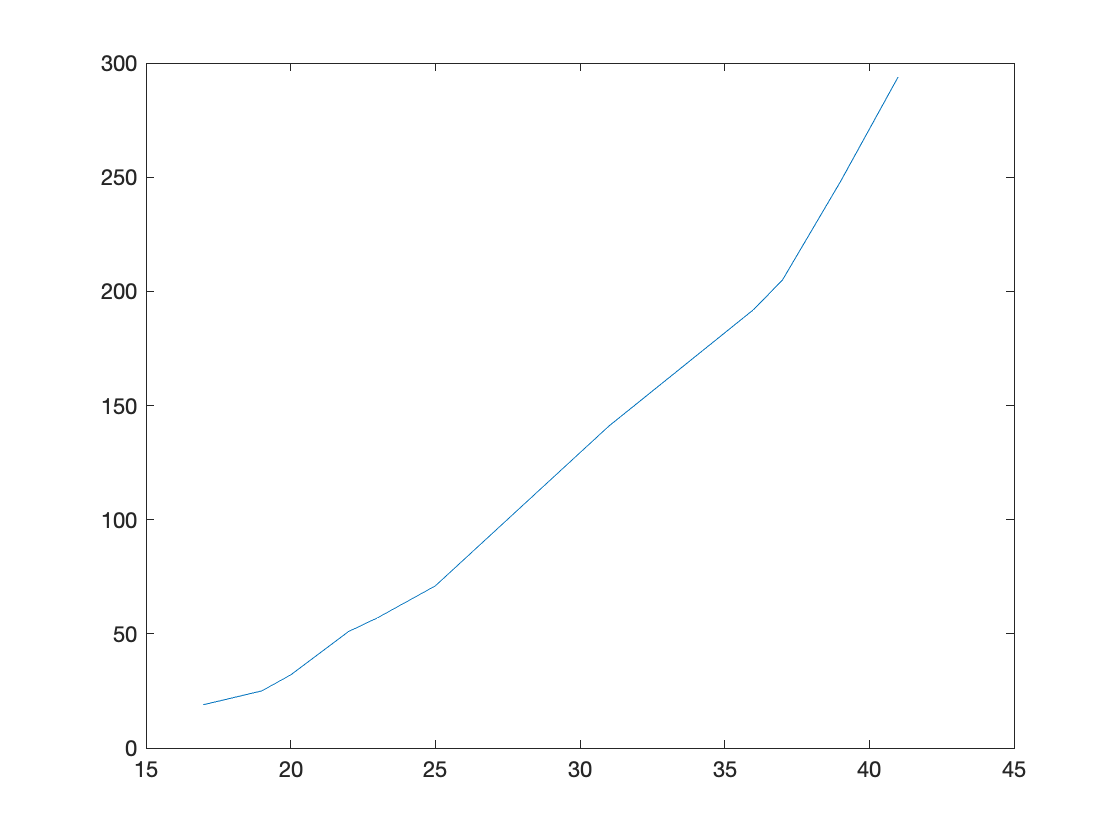
\includegraphics[width=8cm]{figure/2_2.png}
		\caption{After}
		%\label{fig:side:b}
		\end{minipage}
		\end{figure}

		\newpage 
		$\\$The divided difference table for data:\\
		\begin{spacing}{1.5}
		\begin{center}
        \begin{tabular}[b]{cc|ccccccc} 
        $x$ & $y$ & 
        $\Delta y$ & $\Delta^2 y$ & $\Delta^3 y$ & 
        $\Delta^4 y$ & $\Delta^5 y$ & $\Delta^6 y$ & $\Delta^7 y$
        \\
        \hline 
        \makecell{17\\19\\20\\22\\23\\25\\31 \\36 \\37 \\39 \\41 } & 
        \makecell{19\\25\\32\\51\\57\\71\\141\\192\\205\\248\\294} &
        \makecell{3\\7\\9.5\\6\\7\\11.667\\10.2\\13\\21.5\\23} &
     	\makecell{1.3333\\0.8333\\-1.1667\\0.3333\\0.5833\\-0.1333\\0.4667\\2.8333\\0.375}&
     	\makecell{-0.1\\-0.5\\0.3\\0.0278\\-0.0551\\0.05\\0.2958\\-0.4917}&
     	\makecell{-0.0667\\0.1333\\-0.0247\\-0.0059\\0.0075\\0.0176\\-0.0788}&
     	\makecell{0.025\\-0.0132\\0.0012\\0.0009\\0.0006\\-0.006}&
     	\makecell{-0.0027\\0.0008\\-0\\-0\\-0.0004}&
     	\makecell{0.1879$*10^{-3}$\\-0.0478$*10^{-3}$\\0\\-0.0186$*10^{-3}$}
        \end{tabular}
        \end{center}

        \begin{center}
        \begin{tabular}[b]{ccc} 
        
        $\quad$ $\Delta^8 y$ & $\Delta^9 y$ & $\Delta^{10} y$
        \\
        \hline 
        \makecell{}
     	\makecell{-0.1179$*10^{-4}$\\0.0239$*10^{-4}$\\-0.0089$*10^{-4}$}&
     	\makecell{0.6446$*10^{-6}$\\-0.1491$*10^{-6}$}&
     	\makecell{-3.3071$*10^{-8}$}
        \end{tabular}
        \end{center}
        \end{spacing}

        $\\$So I chose the 6-order, 7-order, 8-order and 9-order polynomial to fit this data set :

        \newpage
        \begin{figure}[htbp]
		\centering
		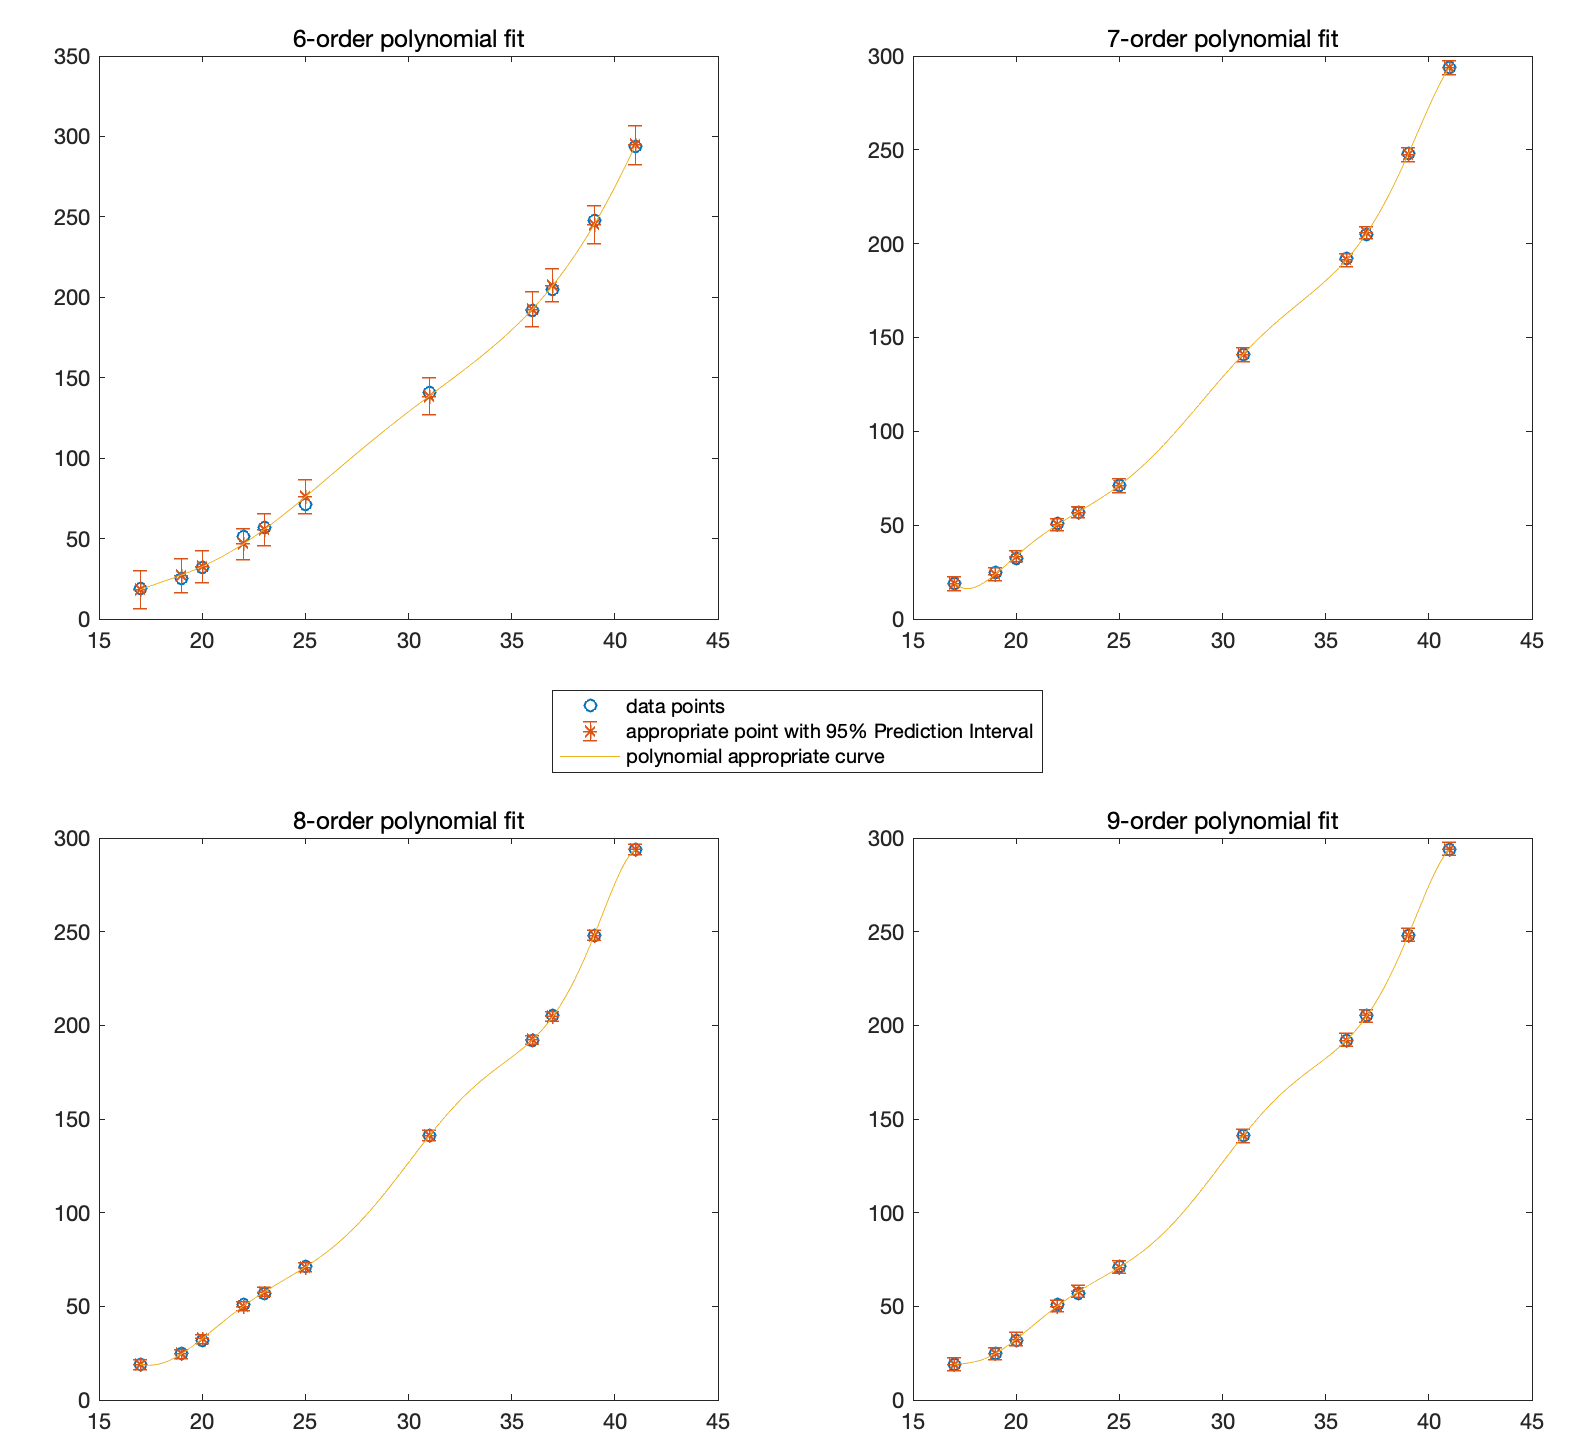
\includegraphics[scale=0.3]{figure/2_3.png}
		\end{figure}

		$\\$
		It is found that the 7-order polynomial is enough to fit this data set.




\end{document}